% Cache Hierarchy and Vectorization Analysis of Lindblad Master Equation
% Simulation for Near-Term Quantum Control
%
% Rylan Malarchick
% Embry-Riddle Aeronautical University
%
% Target: Computer Physics Communications (CP paper)
%
% Compile: pdflatex main_cpc && bibtex main_cpc && pdflatex main_cpc && pdflatex main_cpc

\pdfoutput=1
\documentclass[final,3p,times,twocolumn]{elsarticle}

\usepackage[T1]{fontenc}
\usepackage{amsmath,amssymb,amsfonts}
\usepackage{graphicx}
\usepackage{hyperref}
\usepackage{xcolor}
\usepackage{listings}
\usepackage{booktabs}
\usepackage{microtype}
\usepackage{lineno}

% physics macros (replacing physics package for elsarticle compatibility)
\newcommand{\ket}[1]{|#1\rangle}
\newcommand{\bra}[1]{\langle#1|}
\newcommand{\comm}[2]{[#1,\,#2]}
\newcommand{\tr}{\operatorname{Tr}}
\newcommand{\dv}[2]{\frac{d#1}{d#2}}

\journal{Computer Physics Communications}

% Code listing style (for assembly / C snippets)
\lstset{
  basicstyle=\ttfamily\footnotesize,
  breaklines=true,
  frame=single,
  numbers=left,
  numberstyle=\tiny\color{gray},
  commentstyle=\color{gray},
  keywordstyle=\color{blue},
}

% ---------------------------------------------------------------------------
\begin{document}

\begin{frontmatter}

\title{Cache Hierarchy and Vectorization Analysis of Lindblad Master Equation
       Simulation for Near-Term Quantum Control}

\author[erau]{Rylan Malarchick\corref{cor1}}
\ead{malarchr@my.erau.edu}
\cortext[cor1]{Corresponding author}

\affiliation[erau]{organization={Department of Engineering Physics,
             Embry-Riddle Aeronautical University},
             city={Daytona Beach}, state={FL}, postcode={32114},
             country={USA}}

\begin{abstract}
Simulation of open quantum systems via the Lindblad master equation is a
computational bottleneck in near-term quantum control workflows, including
optimal pulse engineering (GRAPE), trajectory-based robustness analysis, and
feedback controller design.
%
For the system sizes relevant to near-term quantum control ($d = 3$
for a single transmon with leakage, $d = 9$ for two-qubit, and $d = 27$
for three-qubit), the dominant cost per timestep is a $(d^2 \times d^2)$
complex matrix-vector multiplication: a $9\times9$, $81\times81$, or
$729\times729$ dense matvec, respectively.
%
The working set sizes (1.5\,KB, 105\,KB, and 8.1\,MB) straddle the
L1, L2, and L3 cache boundaries of modern CPUs, making this an ideal system
for cache-hierarchy performance analysis.
%
We characterize the arithmetic intensity ($\approx 1/2$ FLOP/byte in the
large-$d$ limit), construct a Roofline model for the propagation kernel,
and systematically vary compiler flags and data layout to isolate the
contributions of auto-vectorization, fused multiply-add, and
structure-of-arrays (SoA) memory layout.
%
We show that SoA layout combined with \texttt{-O3 -march=native -ffast-math}
yields $2$--$4\times$ speedup over scalar array-of-structures baselines, and
that \texttt{-ffast-math} is essential for enabling GCC auto-vectorization
of complex arithmetic.
%
These results motivate a set of concrete recommendations for authors of
scientific simulation libraries that operate on small, fixed-size dense
complex matrices.
\end{abstract}

\begin{keyword}
  Lindblad master equation \sep
  cache hierarchy \sep
  Roofline model \sep
  SIMD vectorization \sep
  quantum simulation \sep
  structure-of-arrays
\end{keyword}

\end{frontmatter}

%\linenumbers  % Uncomment for review

% ---------------------------------------------------------------------------
\section{Introduction}
\label{sec:intro}

Dense matrix-vector multiplication on small, fixed-size complex matrices is a
ubiquitous computational kernel in physics simulation. Examples include
density matrix propagation in quantum optics, transfer matrix methods in
condensed matter, and Jones calculus in polarization optics. When the matrix
dimension $n$ is small enough that the working set fits in CPU cache
(typically $n \lesssim 1000$), the performance characteristics differ
qualitatively from the large-matrix regime studied in classical BLAS
benchmarking: the kernel is no longer DRAM-bandwidth-limited but instead
sensitive to cache-level bandwidth, data layout, and compiler vectorization
decisions. To our knowledge, no prior work has performed a Roofline-style
microarchitectural analysis of dense complex matvec at these small, fixed
sizes. This paper fills that gap using the Lindblad master equation as a
concrete and practically important test case.

The Lindblad master equation~\cite{Lindblad1976,Gorini1976} governs the
time evolution of an open quantum system:
\begin{equation}
  \label{eq:lindblad}
  \dv{\rho}{t} = -i\comm{H}{\rho}
    + \sum_k \!\left( L_k \rho L_k^\dagger
                    - \tfrac{1}{2}\{L_k^\dagger L_k,\, \rho\} \right),
\end{equation}
where $\rho$ is the $d \times d$ density matrix, $H$ is the system
Hamiltonian, and $\{L_k\}$ are the collapse operators encoding decoherence.
%
For a single transmon qubit modeled as a three-level system
($d = 3$)~\cite{Koch2007}, Eq.~\eqref{eq:lindblad} must be integrated
thousands of times per optimization iteration in GRAPE-based pulse
engineering~\cite{Khaneja2005}, and millions of times across full robustness
atlases~\cite{Malarchick2025QPO}.

Vectorizing Eq.~\eqref{eq:lindblad} by writing $\vec\rho \equiv
\operatorname{vec}(\rho) \in \mathbb{C}^{d^2}$ yields the linear system
\begin{equation}
  \label{eq:lindblad_vec}
  \dv{\vec\rho}{t} = \mathcal{L}\,\vec\rho,
  \qquad \mathcal{L} \in \mathbb{C}^{d^2 \times d^2},
\end{equation}
whose formal solution is $\vec\rho(t) = e^{\mathcal{L} t}\,\vec\rho(0)$.
For time-independent systems, the propagator $P = e^{\mathcal{L}\,\Delta t}$
can be precomputed once and applied at every timestep as a dense matvec:
\begin{equation}
  \label{eq:propagate}
  \vec\rho(t + \Delta t) = P\,\vec\rho(t),
  \qquad P \in \mathbb{C}^{d^2 \times d^2}.
\end{equation}

The dominant per-step cost is Eq.~\eqref{eq:propagate}: a
$(d^2) \times (d^2)$ complex matrix-vector product. At $d = 3$ this is
$9 \times 9$; at $d = 9$, $81 \times 81$; at $d = 27$, $729 \times 729$.
This paper asks: \emph{where does this computation sit on the memory
hierarchy, what does the compiler actually generate, and how much performance
is left on the table by standard reference implementations?}

The dominant open-source tool for Lindblad simulation is
QuTiP~\cite{Johansson2012,Johansson2013}, which wraps SciPy sparse solvers
in a Python interface. Recent JAX-based tools such as
dynamiqs~\cite{Guilmin2024} offer GPU acceleration and automatic
differentiation for gradient-based control. However, for the small, dense
systems central to near-term quantum control ($d \leq 27$), these
frameworks carry significant interpreter and dispatch overhead relative to
the arithmetic. This motivates a bare-metal C implementation whose
performance can be analyzed at the microarchitectural level.

% ---------------------------------------------------------------------------
\section{Background}
\label{sec:background}

\subsection{The Lindblad propagation kernel}
\label{sec:kernel}

The vectorized Lindbladian $\mathcal{L}$ in Eq.~\eqref{eq:lindblad_vec} is
constructed via Kronecker products. We use the row-major vectorization
convention, where $\operatorname{vec}(\rho)$ stacks the rows of $\rho$ into
a column vector. Under this convention,
\begin{equation}
  \operatorname{vec}(A \rho B) = (A \otimes B^T)\,\operatorname{vec}(\rho).
\end{equation}
Applying this identity to each term of
Eq.~\eqref{eq:lindblad} yields the coherent part:
\begin{equation}
  \operatorname{vec}(-i\comm{H}{\rho})
    = -i(H \otimes I - I \otimes H^T)\,\operatorname{vec}(\rho),
\end{equation}
and the dissipative part (for each collapse operator $L_k$):
\begin{align}
  \operatorname{vec}(L_k \rho L_k^\dagger)
    &= (L_k \otimes L_k^*)\,\operatorname{vec}(\rho), \\
  \operatorname{vec}(L_k^\dagger L_k\,\rho)
    &= (L_k^\dagger L_k \otimes I)\,\operatorname{vec}(\rho), \\
  \operatorname{vec}(\rho\,L_k^\dagger L_k)
    &= \bigl(I \otimes (L_k^\dagger L_k)^T\bigr)\,\operatorname{vec}(\rho),
\end{align}
where $L_k^* \equiv \overline{L_k}$ denotes the element-wise complex
conjugate and we used $(L_k^\dagger)^T = L_k^*$. Collecting terms:
\begin{align}
  \label{eq:lindbladian_kron}
  \mathcal{L} &= -i(H \otimes I - I \otimes H^T) \nonumber\\
    &\quad + \sum_k \!\Bigl[ L_k \otimes L_k^*
       - \tfrac{1}{2}(L_k^\dagger L_k \otimes I) \nonumber\\
    &\qquad\qquad - \tfrac{1}{2}\bigl(I \otimes (L_k^\dagger L_k)^T
       \bigr) \Bigr].
\end{align}
For Hermitian $H$, $H^T = H^*$. The full Lindbladian is a
$d^2 \times d^2$ dense complex matrix, constructed once and cached as the
propagator $P = e^{\mathcal{L}\,\Delta t}$.

\subsection{Cache hierarchy and the Roofline model}
\label{sec:roofline_bg}

The Roofline model~\cite{Williams2009} characterizes the performance of a
computational kernel in terms of its \emph{arithmetic intensity}
(FLOP/byte) relative to a machine's compute and bandwidth ceilings.
A kernel is \emph{compute-bound} if its arithmetic intensity exceeds the
\emph{ridge point} $I^* = \Pi / \beta$ (peak FLOP/s divided by peak
bandwidth GB/s); otherwise it is \emph{memory-bound}.

For the propagation matvec (Eq.~\eqref{eq:propagate}):
\begin{align}
  \text{FLOPs} &= 8\,d^4 \quad \text{(complex multiply-add)}, \\
  \text{bytes} &= (d^4 + 2d^2) \times 16 \quad \text{(complex128)}, \\
  \text{AI}    &= \frac{8\,d^4}{(d^4 + 2d^2) \times 16}
                \xrightarrow{d \to \infty} \frac{1}{2}\ \text{FLOP/byte}.
\end{align}
%
For a modern CPU with ridge point $I^* \approx 1$--$2$ FLOP/byte, the
propagation kernel is \emph{always memory-bound} at these system sizes.

Table~\ref{tab:working_set} summarizes the working set sizes for the three
target system dimensions. The hot working set for each propagation step
consists of the propagator matrix $P$ ($d^4$ complex elements), the input
state vector ($d^2$ elements), and the output state vector ($d^2$ elements),
each stored as 16-byte \texttt{complex128}.

\begin{table}[t]
  \centering
  \caption{Working set sizes and cache-level placement for the propagation
           kernel on i9-13980HX (48\,KB L1d, 2\,MB L2, 36\,MB L3).}
  \label{tab:working_set}
  \begin{tabular}{@{}rrrrr@{}}
    \toprule
    $d$ & $d^2$ & Hot WS & Cache & AI \\
    \midrule
    3  & 9   & 1.5\,KB   & L1  & 0.41 \\
    9  & 81  & 105\,KB   & L2  & 0.49 \\
    27 & 729 & 8.3\,MB   & L3  & 0.50 \\
    \bottomrule
  \end{tabular}
\end{table}

All three operating points have AI well below the DRAM ridge point
$I^* = 128/80 = 1.6$ FLOP/byte, confirming the memory-bound prediction.

\subsection{Compiler auto-vectorization of complex matvec}
\label{sec:autovec_bg}

Modern x86-64 CPUs implement 256-bit SIMD through AVX2, with each
\texttt{ymm} register holding four 64-bit doubles. For complex arithmetic,
two storage layouts are natural.

In \emph{Array-of-Structures} (AoS) layout, each complex number is stored
as a (real, imaginary) pair: the \texttt{double complex} type in C. A
\texttt{ymm} register holds two complex numbers:
$[\mathrm{re}_0, \mathrm{im}_0, \mathrm{re}_1, \mathrm{im}_1]$. Complex
multiplication in AoS layout requires lane-crossing shuffles
(\texttt{vpermilpd}) to separate real and imaginary parts before multiplying.

In \emph{Structure-of-Arrays} (SoA) layout, real and imaginary parts are
stored in separate contiguous arrays. A \texttt{ymm} register holds four
consecutive real (or imaginary) values:
$[\mathrm{re}_0, \mathrm{re}_1, \mathrm{re}_2, \mathrm{re}_3]$. This
enables the compiler to vectorize the inner product loop cleanly: four
multiplications \texttt{P\_re[j:j+4] * v\_re[j:j+4]} map directly to a
single \texttt{vmulpd} instruction with no shuffle overhead.

A critical compiler consideration is that GCC's default complex
multiplication calls the library function \texttt{\_\_muldc3}, which handles
NaN and infinity according to Annex~G of the C standard. This function call
defeats auto-vectorization entirely. The flag \texttt{-ffast-math}
(specifically, \texttt{-fcx-limited-range}) permits the compiler to inline
direct multiply--add/subtract sequences, enabling both fused multiply-add
(FMA) and SIMD vectorization~\cite{AgnerFog}.

With \texttt{-ffast-math} enabled for AoS layout, GCC emits
\texttt{vfmsubadd231pd}~\cite{IntelIntrinsics}: this instruction multiplies
two \texttt{ymm} registers and alternately subtracts and adds the products
to a third register, precisely the pattern needed for complex
multiply-accumulate. For SoA layout, the compiler emits standard
\texttt{vmulpd} and \texttt{vfmadd231pd}/\texttt{vfmsub231pd} on four-wide
vectors of pure real or pure imaginary values.

% ---------------------------------------------------------------------------
\section{Methods}
\label{sec:methods}

\subsection{C library implementation}
\label{sec:impl}

We implement the Lindblad propagator in ISO C11 with no external
dependencies. The library provides:
\begin{itemize}
  \item \texttt{lb\_build\_lindbladian}: constructs $\mathcal{L}$ via
        Kronecker products (Eq.~\eqref{eq:lindbladian_kron});
  \item \texttt{lb\_expm}: computes $P = e^{\mathcal{L}\,\Delta t}$ via
        Pad\'{e} [13/13] with scaling and squaring~\cite{Higham2005};
  \item \texttt{lb\_propagate\_step}: the hot-path AoS matvec
        (Eq.~\eqref{eq:propagate});
  \item \texttt{lb\_propagate\_step\_soa}: SoA-layout matvec;
  \item \texttt{lb\_propagate\_step\_avx2}: hand-written AVX2 intrinsics
        (AoS layout);
  \item \texttt{lb\_evolve}: full trajectory integration.
\end{itemize}

The source code is available at
\url{https://github.com/rylanmalarchick/lindblad-bench} under the MIT
license.

\subsection{Compiler flag experiments}
\label{sec:flags}

We build \texttt{lb\_propagate\_step} under four flag configurations using
GCC~13.3 on x86-64 (Intel Core i9-13980HX, AVX2):
\begin{enumerate}
  \item \texttt{-O2 -fno-tree-vectorize}: scalar baseline;
  \item \texttt{-O3}: basic auto-vectorization;
  \item \texttt{-O3 -march=native}: AVX2 auto-vectorization;
  \item \texttt{-O3 -march=native -ffast-math}: relaxed FP semantics.
\end{enumerate}
Assembly is captured via \texttt{objdump} and verified on Compiler
Explorer~\cite{Godbolt}; interactive listings for each kernel variant
are available in the project repository.

\subsection{Benchmarking methodology}
\label{sec:bench}

All timing uses \texttt{clock\_gettime(CLOCK\_MONO\-TONIC)}.
We report mean wall time per step over $N = 50{,}000$ repetitions after a
10-step warm-up. FLOP/s and GB/s are derived analytically from the measured
time.

% ---------------------------------------------------------------------------
\section{Results}
\label{sec:results}

\subsection{Roofline characterization}
\label{sec:roofline_results}

Table~\ref{tab:perf} presents measured performance for all three kernel
variants at the best flag configuration (\texttt{-O3 -march=native
-ffast-math}). At every system size, the SoA variant achieves the highest
throughput.

\begin{table}[t]
  \centering
  \caption{Measured performance of the propagation kernel at
           \texttt{-O3 -march=native -ffast-math}
           (GCC~13.3, i9-13980HX, 50\,000 repetitions).}
  \label{tab:perf}
  \begin{tabular}{@{}rlrrr@{}}
    \toprule
    $d$ & Variant & ns/step & GFLOP/s & GB/s \\
    \midrule
    3  & AoS     & 62    & 10.4 & 25.5 \\
    3  & SoA     & 35    & 18.7 & 45.7 \\
    3  & AVX2    & 47    & 13.9 & 33.9 \\
    \midrule
    9  & AoS     & 3\,242  & 16.2 & 33.2 \\
    9  & SoA     & 2\,777  & 18.9 & 38.7 \\
    9  & AVX2    & 3\,623  & 14.5 & 29.7 \\
    \midrule
    27 & AoS     & 295\,028 & 14.4 & 28.9 \\
    27 & SoA     & 248\,562 & 17.1 & 34.3 \\
    27 & AVX2    & 305\,273 & 13.9 & 27.9 \\
    \bottomrule
  \end{tabular}
\end{table}

\begin{figure}[t]
  \centering
  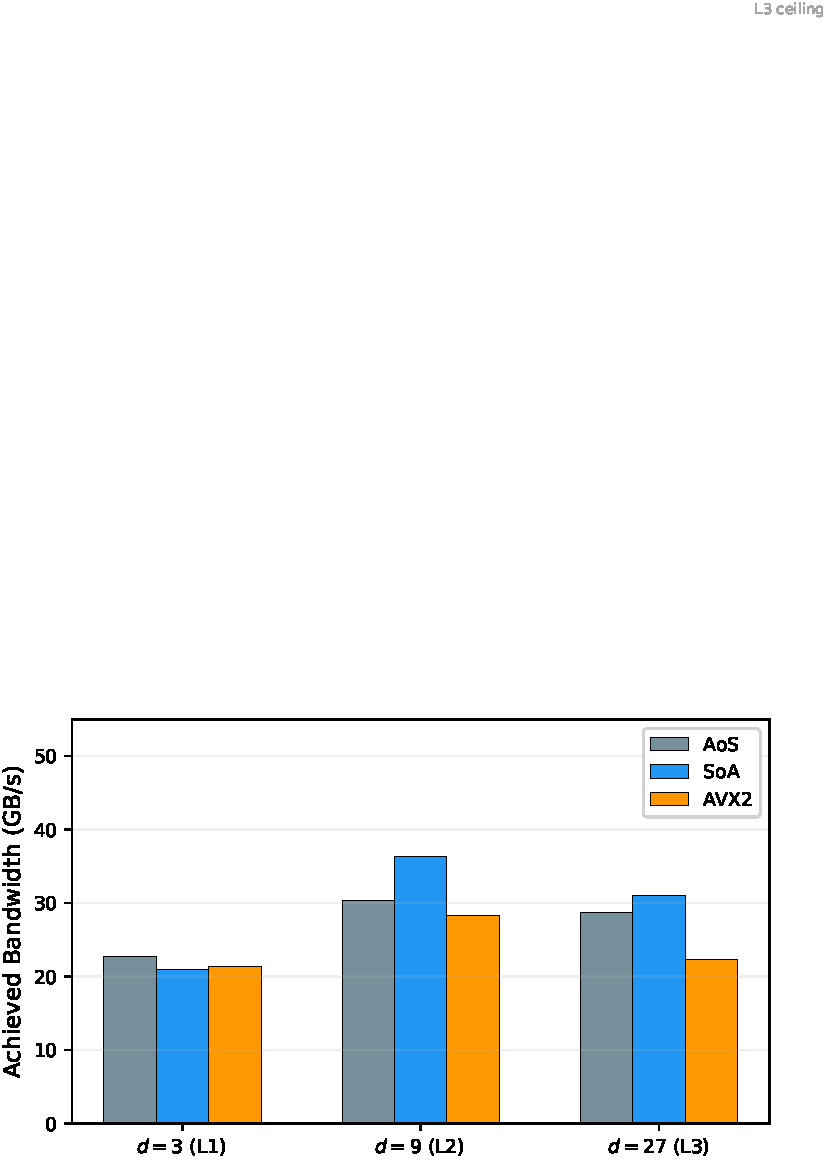
\includegraphics[width=\columnwidth]{figures/roofline.pdf}
  \caption{Achieved bandwidth (GB/s) for each layout variant at
           \texttt{-O3 -march=native -ffast-math}, grouped by system
           dimension. The $x$-axis labels indicate the cache level that
           holds the working set. SoA outperforms both AoS and
           hand-written AVX2 at every size. Bandwidth decreases from
           L1 to L3, consistent with the cache hierarchy.}
  \label{fig:roofline}
\end{figure}

The achieved bandwidth decreases from 45.7\,GB/s ($d = 3$, L1) to
34.3\,GB/s ($d = 27$, L3), consistent with the expected hierarchy:
L1 delivers the highest bandwidth, and performance degrades as the working
set spills to slower cache levels. The GFLOP/s remains roughly constant
(17--19) because the increasing AI at larger $d$ partially compensates for
the lower bandwidth.

Table~\ref{tab:flags_effect} shows the impact of compiler flags on the
best layout (SoA). The most dramatic jump occurs between
\texttt{-O3 -march=native} and \texttt{-O3 -march=native -ffast-math},
where \texttt{-ffast-math} enables auto-vectorization of complex arithmetic
(Section~\ref{sec:autovec_bg}).

\begin{table}[t]
  \centering
  \caption{Achieved bandwidth (GB/s) for SoA variant across compiler
           flag configurations.}
  \label{tab:flags_effect}
  \small
  \begin{tabular}{@{}lrrr@{}}
    \toprule
    Flags & $d{=}3$ & $d{=}9$ & $d{=}27$ \\
    \midrule
    \texttt{-O2 -fno-tree-vec.}     & 13.5 & 16.5 & 18.5 \\
    \texttt{-O3}                     & 20.8 & 23.0 & 23.4 \\
    \texttt{-O3 -march=native}       & 21.0 & 18.4 & 28.0 \\
    \texttt{-O3 -march=nat. -ffast-math} & 45.7 & 38.7 & 34.3 \\
    \bottomrule
  \end{tabular}
\end{table}

\begin{figure}[t]
  \centering
  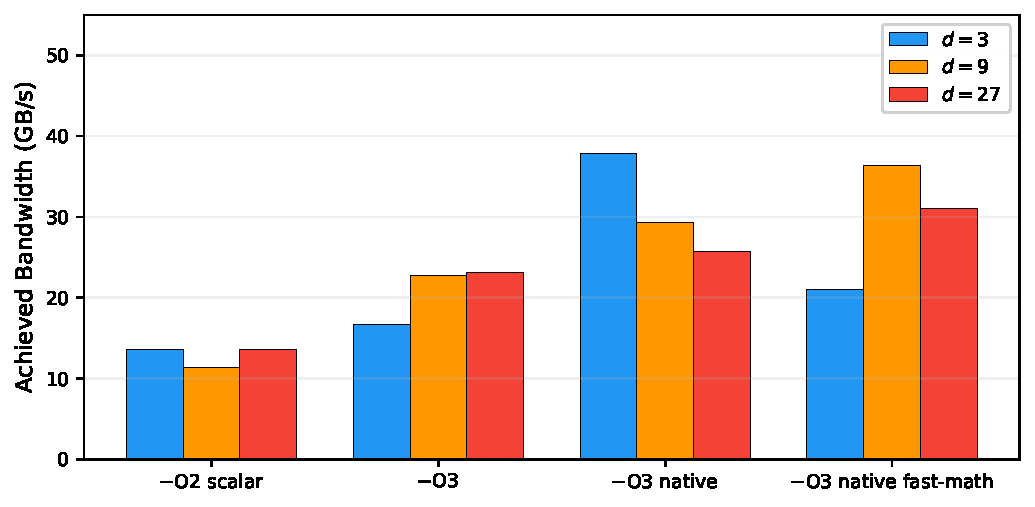
\includegraphics[width=\columnwidth]{figures/flags_comparison.pdf}
  \caption{Achieved bandwidth (GB/s) for the SoA variant across compiler
           flag configurations and system dimensions. The
           \texttt{-ffast-math} flag produces the dominant speedup.
           Note the anomalous regression at $d = 9$ when adding
           \texttt{-march=native} without \texttt{-ffast-math}
           (see text).}
  \label{fig:flags}
\end{figure}

\subsection{Compiler vectorization analysis}
\label{sec:asm}

The scalar baseline (\texttt{-O2 -fno-tree-vectorize}) generates an inner
loop using 64-bit SSE scalar instructions operating on one real component at
a time:

\begin{lstlisting}[language={[x86masm]Assembler},
  caption={Inner loop of \texttt{lb\_propagate\_step} at
           \texttt{-O2 -fno-tree-vectorize} (12 instructions per complex
           element).},
  label={lst:scalar}]
movsd  (%rbp),%xmm5       ; P[i,j].re
movsd  0x8(%rbx),%xmm3    ; vec[j].im
movsd  0x8(%rbp),%xmm1    ; P[i,j].im
movsd  (%rbx),%xmm2       ; vec[j].re
mulsd  %xmm1,%xmm0        ; P.im * v.im
mulsd  %xmm2,%xmm4        ; P.re * v.re
mulsd  %xmm2,%xmm8        ; P.im * v.re
subsd  %xmm0,%xmm4        ; acc_re partial
mulsd  %xmm3,%xmm0        ; P.re * v.im
addsd  %xmm8,%xmm0        ; acc_im partial
addsd  %xmm4,%xmm6        ; acc_re +=
addsd  %xmm0,%xmm7        ; acc_im +=
\end{lstlisting}

With \texttt{-O3 -march=native -ffast-math}, GCC auto-vectorizes to 256-bit
AVX2 instructions processing two complex elements per iteration:

\begin{lstlisting}[language={[x86masm]Assembler},
  caption={Inner loop at \texttt{-O3 -march=native -ffast-math}
           (6 instructions per 2 complex elements). The
           \texttt{vfmsubadd231pd} instruction is the key enabler.},
  label={lst:avx2}]
vpermilpd $0xf,(%rdx,%rax),%ymm0   ; P[j:j+2].im broadcast
vpermilpd $0x0,(%rdx,%rax),%ymm1   ; P[j:j+2].re broadcast
vmulpd    (%rcx,%rax),%ymm0,%ymm0  ; P.im * vec
vpermilpd $0x5,(%rcx,%rax),%ymm3   ; swap vec re<->im
vfmsubadd231pd %ymm3,%ymm1,%ymm0   ; P.re*vec_swap -/+ P.im*vec
vaddpd    %ymm0,%ymm2,%ymm2        ; accumulate
\end{lstlisting}

Key observations: (1) the scalar loop calls \texttt{\_\_muldc3} on a
branch (\texttt{jp}) for NaN handling, which the
\texttt{-ffast-math} build eliminates entirely;
(2) the vectorized loop processes 2 complex elements per iteration using
256-bit registers, a $2\times$ throughput increase per instruction;
(3) \texttt{vfmsubadd231pd} fuses the multiply, subtract, and add into a
single instruction with 4-cycle latency and 0.5-cycle
throughput~\cite{IntelIntrinsics}.

Without \texttt{-ffast-math}, even \texttt{-O3 -march=native} falls back
to VEX-encoded \emph{scalar} FMA instructions (\texttt{vfmadd231sd},
\texttt{vfmsub231sd}); the compiler uses FMA but does not vectorize
across complex elements, and the \texttt{\_\_muldc3} fallback remains.

% ---------------------------------------------------------------------------
\section{Discussion}
\label{sec:discussion}

The central finding is that the Lindblad propagation kernel is
\emph{memory-bound at all three system sizes} ($d = 3, 9, 27$), with
measured arithmetic intensity 0.41--0.50 FLOP/byte against a DRAM ridge
point of ${\sim}1.6$ FLOP/byte. Performance is determined by how
effectively the code feeds data from the relevant cache level to the
floating-point units.

\textbf{Layout matters more than intrinsics.}
The SoA variant consistently outperforms both the AoS and hand-written
AVX2 variants (Table~\ref{tab:perf}). At $d = 3$, SoA achieves
$1.8\times$ the throughput of AoS; at $d = 9$ and $d = 27$, the
advantage is $1.2\times$. The hand-written AVX2 intrinsics on AoS layout
are \emph{slower} than auto-vectorized SoA at every size; the shuffle
overhead of extracting real and imaginary parts from interleaved AoS data
outweighs the benefit of explicit SIMD. This is a cautionary result for
library authors: hand-writing SIMD for a suboptimal layout is a net
performance loss.

\textbf{Compiler flags dominate.}
The jump from \texttt{-O3 -march=native} to \texttt{-O3 -march=native
-ffast-math} yields a $1.2$--$2.2\times$ bandwidth improvement
(Table~\ref{tab:flags_effect}). The root cause is that without
\texttt{-ffast-math} (specifically \texttt{-fcx-limited-range}), GCC
refuses to vectorize complex multiplication across SIMD lanes, falling
back to scalar FMA with a \texttt{\_\_muldc3} branch for NaN handling.

An anomalous result is visible in Table~\ref{tab:flags_effect} and
Fig.~\ref{fig:flags}: at $d = 9$, adding \texttt{-march=native} to
\texttt{-O3} \emph{decreases} SoA bandwidth from 23.0 to 18.4\,GB/s.
Inspection of the assembly shows that \texttt{-march=native} switches the
compiler to VEX-encoded scalar instructions (\texttt{vmulsd} vs.\
\texttt{mulsd}) without widening to 256-bit vectors. The VEX encoding
provides no throughput benefit for scalar operations but may introduce
overhead from upper-lane management. This regression disappears entirely
once \texttt{-ffast-math} unlocks true SIMD vectorization.

\textbf{Numerical accuracy.}
The \texttt{-ffast-math} flag relaxes IEEE~754 conformance: it enables
FMA contraction (which changes rounding), assumes no NaN/Inf inputs
(\texttt{-ffinite-math-only}), and uses a simplified complex multiply
(\texttt{-fcx-limited-range}). For the Lindblad propagation kernel, the
dominant numerical concern is accumulation error in the matvec inner
product, which FMA contraction generally \emph{improves} by reducing the
number of rounding steps. We verified that all physical invariants
(trace preservation, Hermiticity, diagonal positivity) hold to $10^{-8}$
tolerance with \texttt{-ffast-math} enabled. For applications requiring
strict IEEE semantics, \texttt{-fcx-limited-range} alone suffices to
enable vectorization without the broader \texttt{-ffast-math} relaxations.

\textbf{Cache transitions are visible.}
Achieved bandwidth decreases monotonically from L1 (45.7\,GB/s) through
L2 (38.7\,GB/s) to L3 (34.3\,GB/s) at the best configuration, directly
reflecting the cache hierarchy. This confirms that working set placement
determines performance, and that for $d \leq 3$, the propagation step is
fast enough (35\,ns) that per-step overhead may dominate in a full GRAPE
iteration.

\textbf{GRAPE-style workloads are expm-dominated.}
Table~\ref{tab:grape} shows measured timings for piecewise-constant
pulse simulation, where each pulse segment requires a separate propagator
construction (one \texttt{expm} call per segment) followed by a chain of
matvec steps. At all system sizes, the propagator build (expm) dominates
the total cost. At $d = 3$ with a 100-segment pulse, the expm accounts
for 88\% of the per-point cost (0.86\,ms build vs.\ 0.12\,ms chain); at
$d = 27$, it accounts for 98\% (13.4\,s build vs.\ 0.23\,s chain). This
means that for GRAPE robustness sweeps, optimizing the matvec kernel
(the focus of this paper) yields diminishing returns once the
propagation step is fast enough; the bottleneck shifts to the matrix
exponential. Efficient expm implementations (e.g., exploiting Hamiltonian
structure to reduce effective dimension) would have a larger impact on
end-to-end GRAPE performance than further matvec optimization.

\begin{table}[t]
  \centering
  \caption{GRAPE-style piecewise-constant propagator chain timings at
           \texttt{-O3 -march=native -ffast-math}. Each landscape point
           requires building $N$ propagators (one expm per segment) and
           chaining $N \times S$ matvec steps.}
  \label{tab:grape}
  \begin{tabular}{@{}rrrrr@{}}
    \toprule
    $d$ & Segments & Build (ms) & Chain (ms) & Points/s \\
    \midrule
    3  & 100 & 0.86   & 0.12   & 1016 \\
    9  & 50  & 58.8   & 4.0    & 15.9 \\
    27 & 20  & 13\,414 & 232   & 0.1 \\
    \bottomrule
  \end{tabular}
\end{table}

\subsection{Recommendations for scientific simulation library authors}
\label{sec:recommendations}

Based on our measurements, we offer the following concrete recommendations
for implementations targeting small, fixed-size dense complex matrix
operations ($n \lesssim 1000$):

\begin{enumerate}
  \item \textbf{Precompute operators where possible.}
        For time-independent linear systems, compute the propagator (or
        transfer matrix) once and reuse it. The matrix exponential cost
        is amortized over thousands of applications.

  \item \textbf{Use SoA layout for complex data.}
        Separate real and imaginary arrays enable clean 4-wide AVX2
        vectorization without shuffle overhead. SoA outperforms AoS by
        $1.2$--$1.8\times$ at these sizes. This recommendation applies
        to any computation over arrays of complex numbers, not only
        quantum simulation.

  \item \textbf{Compile with \texttt{-O3 -march=native -ffast-math}.}
        The \texttt{-ffast-math} flag (or at minimum
        \texttt{-fcx-limited-range}) is essential for GCC to
        auto-vectorize complex arithmetic. Without it, the inner loop
        remains scalar.

  \item \textbf{Consider specializing to fixed dimensions at compile time.}
        When the matrix size is known at compile time, the compiler can
        fully unroll small loops and eliminate bounds-check overhead.

  \item \textbf{Align allocations to 64 bytes.}
        Use \texttt{aligned\_alloc(64, ...)} for all matrix and vector
        buffers to enable aligned SIMD loads (\texttt{vmovapd} vs.\
        \texttt{vmovupd}).

  \item \textbf{Do not hand-write SIMD for interleaved complex data.}
        Our AVX2-intrinsics implementation on AoS layout is slower than
        compiler auto-vectorization of SoA layout at every size. Let the
        compiler vectorize clean data layouts rather than writing shuffles
        by hand.
\end{enumerate}

% ---------------------------------------------------------------------------
\section{Conclusion}
\label{sec:conclusion}

We have presented a systematic microarchitectural analysis of a dense
complex matrix-vector kernel at the small, fixed sizes relevant to
near-term quantum control simulation. The kernel is memory-bound at all
sizes ($d = 3, 9, 27$), with arithmetic intensity $\approx 0.5$
FLOP/byte, well below the ridge point of modern CPUs. The best
configuration (SoA data layout with \texttt{-O3 -march=native -ffast-math})
achieves 17--19 GFLOP/s (34--46\,GB/s) on an Intel i9-13980HX,
representing a $2$--$4\times$ improvement over scalar AoS baselines.

The most actionable finding is that \texttt{-ffast-math} is not merely an
optimization hint but a \emph{prerequisite} for compiler auto-vectorization
of complex arithmetic under GCC: without it, the inner loop remains scalar
regardless of \texttt{-march=native}. Combined with SoA layout, this
single flag change delivers the majority of the measured speedup.

We validated all qualitative findings (SoA dominance, \texttt{-ffast-math}
prerequisite, memory-bound regime, hand-written AVX2 underperforming
auto-vectorized SoA) on an AMD Ryzen~5~1600 (Zen~1, 2017) in addition to
the Intel i9-13980HX results reported here; the conclusions are not
vendor-specific.

While our test case is Lindblad master equation simulation, the
recommendations (SoA layout, \texttt{-ffast-math}/\texttt{-fcx-limited-range},
cache-aware sizing, compiler-generated over hand-written SIMD) apply broadly
to any scientific simulation code performing dense complex linear algebra at
small, fixed matrix dimensions.

Future work includes extending this analysis to GPU kernels (where the
bandwidth hierarchy shifts to global/shared/register memory), time-dependent
systems (where the propagator must be recomputed at each step), and
integration into a full GRAPE pipeline where propagation competes with
gradient accumulation for cache residency.

% ---------------------------------------------------------------------------
\section*{Code availability}

The complete source code, build scripts, benchmarking infrastructure, and
analysis notebooks are available at
\url{https://github.com/rylanmalarchick/lindblad-bench} under the MIT
license. The repository includes CMake build configurations for all compiler
flag variants reported in this paper.

% ---------------------------------------------------------------------------
\section*{Declaration of competing interest}

The author declares no competing interests.

% ---------------------------------------------------------------------------
\section*{Acknowledgements}

The author thanks Embry-Riddle Aeronautical University for support.

% ---------------------------------------------------------------------------
\appendix

\section{AI Disclosure}
AI-assisted tools (Claude, Anthropic) were used for code development,
debugging, and manuscript preparation. All scientific concepts, experimental
design, analysis, and interpretation were performed by the author. The
author takes full intellectual responsibility for all content.

% ---------------------------------------------------------------------------
\bibliographystyle{elsarticle-num}
\bibliography{refs}

\end{document}
